



\subsection{Participants}
The participants were 132 students from Boğaziçi University who are native speakers of Turkish. In exchange for their participation, they received 1 point to their overall course score with the consent of the course's instructor.

\subsection{Materials}

I used the environment I introduced in the previous section and altered the disambiguation and parallelism between the conjuncts. I provide the template for an experimental item in (\ref{constemplate})(`W' stands for `word', abbreviated because of space limitations).

\begin{exe}
\ex \label{constemplate}
[1W] CONJ1 and CONJ2-{\Case} [2W] PRONOUN [1W] MainVerb
\end{exe}

The pronoun is the factor of Disambiguation with levels: Subject and Object. In Subject, \textit{birbirlerin-{\Case}} `each\_other' disambiguates towards a no SA reading. In Object, \textit{onlar-{\Case}} `{\Tpl}' disambiguates towards an SA reading. The factor Parallelism has two levels: Parallel and Non-parallel. In Parallel, the conjoiner is immediately followed by a noun. In Non-parallel, the conjoiner is followed by an adjective first and then a noun. In (\ref{exp3conditions}), I give partial sentences for all the experimental conditions.
\begin{exe}
\ex \label{exp3conditions}
\begin{xlist}
    \ex Subject, Parallel\\* 
    \gll {\ldots} [baron] ve [şövalye-yi {\ldots} kral] birbirlerini {\ldots} dinle-yecek. \\ 
    {\ldots} baron {\And} knight-{\Acc} {\ldots} king each\_other {\ldots} listen-{\Fut} \\
    \glt `{\ldots} [the baron] and [the king who {\ldots} the knight] will listen to each other {\ldots}'
    
    \ex Subject, Non-parallel\\* 
    \gll {\ldots} [baron] ve [cesur şövalye-yi {\ldots} kral] birbirlerini {\ldots} dinle-yecek. \\ 
    {\ldots} baron {\And} bold knight-{\Acc} {\ldots} king each\_other {\ldots} listen-{\Fut} \\
    \glt `{\ldots} [the baron] and [the king who {\ldots} the bold knight] will listen to each other {\ldots}'
    
    \ex Object, Parallel\\* 
    \gll {\ldots} [baron ve şövalye-yi] {\ldots} kral onları {\ldots} dinle-yecek. \\ 
    {\ldots} baron {\And} knight-{\Acc} {\ldots} king {\Tpl} {\ldots} listen-{\Fut} \\
    \glt `{\ldots} the king who {\ldots} [the baron and the knight] will listen to them {\ldots}'
    
    \ex Object, Non-parallel\\*
    \gll {\ldots} [baron ve cesur şövalye-yi] {\ldots} kral onları {\ldots} dinle-yecek. \\ 
    {\ldots} baron {\And} bold knight-{\Acc} {\ldots} king {\Tpl} {\ldots} listen-{\Fut} \\
    \glt `{\ldots} the king who {\ldots} [the baron and the bold knight] will listen to them {\ldots}'
\end{xlist}
\end{exe}

After every sentence, a statement was presented and the participants judge if the statement was true or false depending on the sentence they read. The statement targeted the theta role assignments. It had two types. One that was only true with SA (Object conditions), meaning that the first conjunct held theta role relation with the embedded verb. The other was only true with no SA (Subject conditions), meaning that the first conjunct held theta role relation with the matrix verb. For the full list of sentences (items 1-40, fillers 101-180) and questions (items 1-40, fillers 101-180) see Appendix \ref{equivalanceitems}

\begin{exe}
\ex \label{exp3qtype}
\begin{xlist}
    \ex Subject true (no SA)\\* 
    \gll Baron kral-ı {\ldots} dinle-yecek. \\ 
    Baron[{\Nom}] king-{\Acc} {\ldots} listen-{\Fut}[{\Tsg}] \\
    \glt `The baron will listen to the king {\ldots}'

    \ex Object true (SA)\\* 
    \gll Kral baron-u ödüllendir-miş \\ 
    King[{\Nom}] baron-{\Acc} reward-{\Prf}[{\Tsg}] \\
    \glt `The king {\ldots} the baron.'
\end{xlist}
\end{exe}

\subsection{Procedure}

Participants were provided with a link to the experiment prompting them with a consent page. Upon giving consent, the participants went through 5 practice items and then they were prompted again for the beginning of the experiment. Each trial proceeded by the participants pushing the `space' key, for each key stroke a word at the center of the screen appeared and by each key stroke it was replaced with the following word in the sentence. After the sentence was read, the participants were presented with a statement that was either true or false according to the sentence they read. They professed their decision by pushing `Q' key for `yes' and `P' key for `no' on the keyboard. The experiment only recorded word reading times, responses, and response times. After the experiment was done, the participants were redirected to a separate page where they provided their student information to be relayed to the course's professor for the extra credit. This is kept separate of the experiment results, keeping participant information and experimental data anonymous.

\subsection{Results}

The results were recorded onto a csv file and imported into R \citep{team2013r} for data cleaning, aggregation, and analysis. The data consisted of 140714 data points. 1 subject with accuracy lower than 70\% in filler items is excluded from the data. The trials which had a word with reading times outside 100-3000 milliseconds are considered as outliers and also excluded. These exclusions resulted in the loss of 8.17\% of the data. In Figure \ref{fig:exp3sentenceread}, I give the average reading times per word with a representative sentence.


\begin{knitrout}
\definecolor{shadecolor}{rgb}{0.969, 0.969, 0.969}\color{fgcolor}\begin{figure}[hbt!]

{\centering 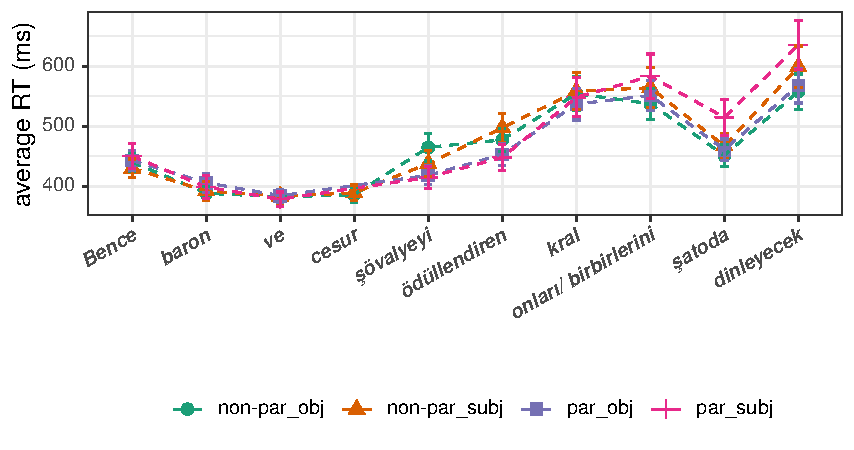
\includegraphics[]{experiments/equivalance/report/figure/exp3sentenceread-1.pdf} 

}

\caption[Third experiment, average reading times of words for all experiment conditions by Disambiguation(Subject, Object) and Parallelism(Parallel, Non-parallel)]{Third experiment, average reading times of words for all experiment conditions by Disambiguation(Subject, Object) and Parallelism(Parallel, Non-parallel)}\label{fig:exp3sentenceread}
\end{figure}


\end{knitrout}

The critical region in all the sentences is the Disambiguation word \textit{onlar-{\Case}} or \textit{birbirlerin-{\Case}}. The spillover region in all the sentences is the two words after the Disambiguation word. In the case of Figure \ref{fig:exp3sentenceread} it is the two words \textit{şatoda} `at the chateau' and \textit{dinleyecek} `will listen'. I give the average RTs of critical and spillover regions in Figure \ref{fig:exp3critandso}. On average, Subject and Parallel conditions result in higher RTs.

\begin{knitrout}
\definecolor{shadecolor}{rgb}{0.969, 0.969, 0.969}\color{fgcolor}\begin{figure}[hbt!]

{\centering 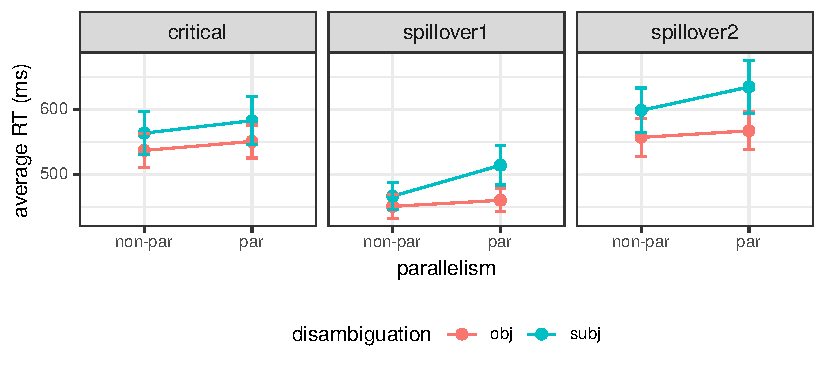
\includegraphics[]{experiments/equivalance/report/figure/exp3critandso-1.pdf} 

}

\caption[Third experiment, average reading times of critical and spillover regions by Disambiguation(Subject, Object) and Parallelism(Parallel, Non-parallel)]{Third experiment, average reading times of critical and spillover regions by Disambiguation(Subject, Object) and Parallelism(Parallel, Non-parallel)}\label{fig:exp3critandso}
\end{figure}


\end{knitrout}

For more inference in RTs in critical and spillover regions, I fit a regression model using brms package in R \citep{burkner2017brms}. I used sum contrasts for the predictors and controlled for the random effects for participant and experimental item. I give the results of the models in Figure \ref{fig:exp3critandsomodel}. The model results indicate that Subject and Parallel conditions have a main effect of increasing RTs. They are more pronounced in the spillover region.

\begin{knitrout}
\definecolor{shadecolor}{rgb}{0.969, 0.969, 0.969}\color{fgcolor}\begin{figure}[hbt!]

{\centering 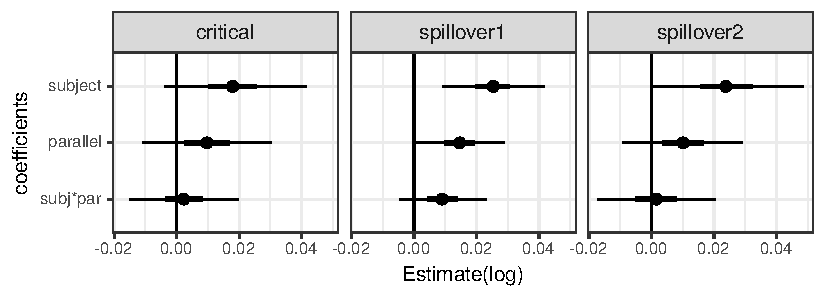
\includegraphics[]{experiments/equivalance/report/figure/exp3critandsomodel-1.pdf} 

}

\caption[Third experiment, model results of RTs for critical and spillover regions with the predictors Disambiguation(Subject, Object) and Parallelism(Parallel, Non-parallel)]{Third experiment, model results of RTs for critical and spillover regions with the predictors Disambiguation(Subject, Object) and Parallelism(Parallel, Non-parallel)}\label{fig:exp3critandsomodel}
\end{figure}


\end{knitrout}

In Figure \ref{fig:exp3accuracy}, I give participant accuracies grouped by experiment conditions and correct answer type. On average, participant accuracies are high in Object conditions and when the correct answer is `yes'. There is an interaction between the correct answer `no' and the Subject conditions where the accuracies are considerably lower.

\begin{knitrout}
\definecolor{shadecolor}{rgb}{0.969, 0.969, 0.969}\color{fgcolor}\begin{figure}[hbt!]

{\centering 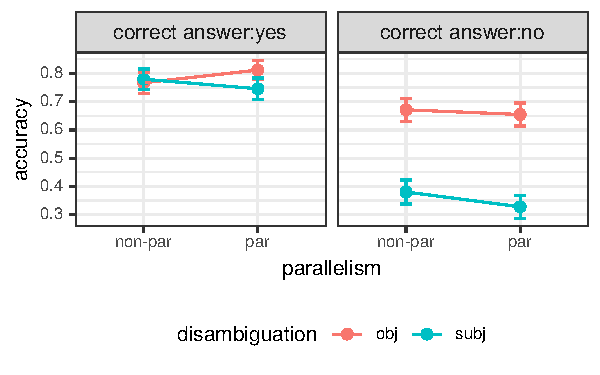
\includegraphics[]{experiments/equivalance/report/figure/exp3accuracy-1.pdf} 

}

\caption[Third experiment, average participant accuracy by Disambiguation(Subject, Object) and Parallelism(Parallel, Non-parallel)]{Third experiment, average participant accuracy by Disambiguation(Subject, Object) and Parallelism(Parallel, Non-parallel)}\label{fig:exp3accuracy}
\end{figure}


\end{knitrout}

For more inference in response accuracy, I fit a regression model using brms in R. This time, the correct answer type is added to the predictors. All predictors have sum contrasts and I controlled for random effects of subject and item. I give the model results in Figure \ref{fig:exp3accuracymodel}.

\begin{knitrout}
\definecolor{shadecolor}{rgb}{0.969, 0.969, 0.969}\color{fgcolor}\begin{figure}[hbt!]

{\centering 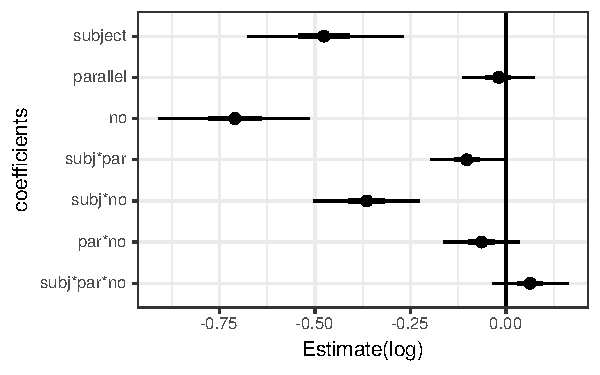
\includegraphics[]{experiments/equivalance/report/figure/exp3accuracymodel-1.pdf} 

}

\caption[Third experiment, model results for subject accuracies fit to responses with the predictors Disambiguation(Subject, Object), Parallelism(Parallel, Non-parallel), and Correct Answer(yes, no)]{Third experiment, model results for subject accuracies fit to responses with the predictors Disambiguation(Subject, Object), Parallelism(Parallel, Non-parallel), and Correct Answer(yes, no)}\label{fig:exp3accuracymodel}
\end{figure}


\end{knitrout}


\subsection{Analysis}

I evaluate the results of the experiment in two parts. In the first part, I analyze the changes in RTs. In the second part I analyze the changes in response accuracies. 

\subsubsection{Analysis of reading times}

Subject conditions result in higher RTs than Object conditions. This means that the parser have gone through a process that costs extra effort in Subject conditions. These conditions require having no suspension of {\Case}. Increase in Subject conditions means that the initial reading was compatible with an SA interpretation but it was changed. This indicates suspension taking place in local environments, no matter what the structural ambiguity in the sentence as a whole is. This is a Reanalysis effect directly related to SA and how the parser operates when it is possible to perform SA.

Parallel conditions display higher RTs than non-parallel conditions. There is no structural ambiguity that the effect can be attributed to. In both levels of Disambiguation, accessing a conjunction is required for establishing antecedents for the pronoun. There is an interaction between the levels Subject and Parallel in the first spillover word, suggesting an increase in difficulty. In Subject conditions, the conjunction needs to be accessed and then broken apart. After this operation, a new conjunction is formed. This first noun and the head noun of the relative clause are conjoined as subjects.

Parallel conditions do not have any contrast between the conjuncts whereas non-parallel conditions have the second conjunct modified by an adjective. This creates a contrast between the conjuncts. Marked conjuncts being more accessible for retrieval has been shown previously \citep{Hofmeister2014} and similarity effects for establishing dependencies are also attested (see \citet{Jager2017} for a review). In Subject conditions, the conjunction to be broken apart needs to be retrieved, and the first noun needs to be taken out the conjunction. Addressing the correct noun in memory becomes harder in parallel conjuncts. This breaking process may be an effect of $dechunking$ \citet{martin2011direct}.

There is a main effect of Parallelism, relatively stable in all regions. It is more pronounced, as the interaction effect, in the first spillover word. I do not see an inherent reason for why parallel conjuncts increased difficulty. It is actually shown to facilitate processing in conjunctions \citep{frazier2000processing}, yet here it displays an opposite effect. The parallelism tested in \citep{frazier2000processing} is not a target to be broken apart or establishing antecedent relations with. 

The only thing common in the pronouns that are used for Disambiguation is their number marking. They are both marked {\Pl} but there is no plural noun among the possible antecedents. The pronoun number agrees with a complex number feature that takes the number of conjuncts instead of the number markings on nouns. Plural agreement is not obligatory in Turkish for conjoined nouns so there is no incentive to form a {\Pl} value for a conjunction when it is formed. I speculate that the easier it is to form a conjunction, the harder it gets to address its parts for establishing a complex feature for number. This is the main effect that is observed in my experiment. Parallel conjuncts are easier to form, average reading differences on the second conjunct \textit{şövalyeyi} in Figure \ref{fig:exp3sentenceread} and a regression model with only Parallelism as the predictor (median log estimate -0.027, \%50 CI -0.032--0.021, \%95 CI -0.042--0.011) confirms the processing ease of parallel conjuncts. This makes it harder to access their parts in forming a complex feature for the conjunction since each of the conjuncts needs to be checked for the number feature. It even makes it harder to break the conjunction apart and form a new one.


\subsubsection{Analysis of response accuracies}

The participants were given a statement to judge depending on the sentence they read. This makes the statement a memory probe for which the participants search compatible readings in their memories. A match results in answering with `Yes' and a lack of finding a match results in answering with `No'. 

Subject conditions decrease participant accuracies overall. In Subject conditions, there was a point of Reanalysis. Overall decrease in Subject conditions mean that either the Reanalysis was not carried out even if it was, the statement was still judged erroneously. There is an interaction between the level Subject and `No' as the correct answer. This means that when the participants were supposed to answer with `No' in Subject conditions, they performed worse compared to Object conditions or `Yes' as the correct answer. This interaction can be attributed to matching the statement to a reanalyzed reading in the memory. When the statement is taken to be a memory probe, the participant had two readings formed, one that is actually true and one that was reanalyzed. The existence of both readings in the memory makes both statement types to have a match thereby decreasing accuracy further when the statement is indeed false. This is in line with the studies that show readings being addressable in memory \citep{christianson2001thematic,van2006activation,Slattery2013} even after Reanalysis.

When the statement was indeed false and the participants were supposed to answer with `No', they performed lower in general compared to the statements that were indeed true. When the statement is taken to be a memory probe for finding a match in memory, answering with `No' becomes the result of an exhaustive search that requires checking all available readings. This exhaustive operation might result in parser abandoning the search and give a random answer, possibly biased towards yes. Remember that not all statements are made about the theta role assignments and false statements only make up 1/4 of the questions. This reduces the chances of conditioning the parser for the task \citep{Swets2008,logavcev2016multiple}. 

Parallel conjuncts do not have a main effect and only have interaction effects with Subject and `No' as correct answer. It reduced accuracy in both. The main effect of increased difficulty in reading times seem to have effected Subject conditions more than they did Object conditions. It was shown that Subject and Parallel conditions had an interaction in the first word of the spillover. Subject conditions included a process of Reanalysis. The difficulty of breaking the conjunction combined with the Reanalysis might have proven too much for the parser, and lead to misparsing hence the interaction effect. In object conditions though, this increased difficulty did not lead to misparsing and that is why a main effect of Parallel seems to be lacking (although the median estimate and \%50 credible intervals are below zero indicating a relatively decrease in accuracy). All the effects of Subject and `No' as correct answer, and interaction with parallel decreasing accuracies are compatible with good enough approach \citep{ferreira2001misinterpretations,ferreira2007good} that suggests language input is not strictly implemented during processing. Partially satisfied relations are taken to be enough if the required effort exceeds the resources that the parser is needed to allocate. 


\section{Discussion}

The second experiment showed that suspension of a suffix is costly, yet this experiment has shown that it is a preferred operation. A deterministic serial parser can predict this, as long as it filters possible conjunctions for {\Case} match and carry out any process necessary to satisfy it to keep the structure minimal. A probabilistic serial parser can predict this result as well, considering that suspension takes less processing resources (thereby time) than positing an embedded clause. The results further indicate that the participants did not fully interpret the sentences when the processing cost proved higher than expected.

In the experiment, the ambiguity environments did not use only {\Acc} to be reconstructed, there were examples of {\Dat}, {\Loc}, and {\Abl} in similar numbers. These can fall into different categories of {\Case} \citep{woolford2006lexical} and their category is only apparent when a verb is reached. Thereby {\Case} can play both a syntactic and a semantic role. If thematic roles are preemptively assigned by {\Case}, then the participants should have favored no SA reading. Some studies in German \citep{gorrell2000subject,schlesewsky2000subject,bader2000reanalyis} show that ambiguous {\Case} markings on arguments receive preferred readings of subject over object. The preferred reading is compatible with an SOV ordering just like the canonical word order in Turkish. None of those studies employ an example of {\Case} ambiguity in a conjunction where both the subject ({\Nom}) and the internal argument ({$\neg$\Nom}) {\Case} markings are available by means of SA. Another difference is that {\Case} is decomposable in Turkish, and no {\Case} marking is ambiguous. Even when the first conjunct was marked with {\Nom} and canonical word order being SOV in Turkish, the participants favored a reading that is incompatible with the {\Nom} or Subject interpretation. There is one crucial point in this experiment. To prevent information structure driven effects, I placed the nominative marked noun not in a sentence initial position, but following a speech act adverbial. This might have prevented the information like SOV word order to be used.


\section{Conclusion}

The results and the analysis indicate that people still perform SA of {\Case} even when it is made ambiguous. Conjunct parallelism do not regulate performing SA or not, but it effects the cost of Reanalysis. This experiment has shown that {\Case} information is overwritten for the sake of positing minimal structures, or structures that take less time to build. This means that the parser favors syntactically simple structures to morphologically complex operations.

The effects of {\Case} for processing ambiguities of conjunctions received very little attention in the literature. The only relevant study I could find was \citet{Traxler1996} where the {\Case} ambiguous `you' in English is contrasted to the unambiguous pronouns for predicting the attachment for c-selection ambiguous verbs like `recognize' that can have both a sentence and a noun as their internal argument. That study concludes in participants using {\Case} information rapidly and effectively. A similar but different story holds for this experiment, the {\Case} is updated in local environments of conjunction. Breaking this update is costly or even not done properly after a contradicting information is encountered.
